\begin{frame} 
	\frametitle{Computing speed from the measurements of position} 
	Consider a car and a (quite inaccurate) model of it
	\begin{columns}[onlytextwidth]
		\column{.4\textwidth}
		\begin{figure}[h]
			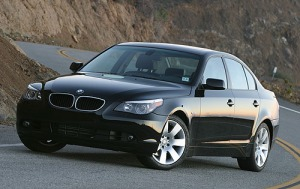
\includegraphics[width=\textwidth]{fig/auto_real}%
			\caption*{The car we want to model.\footnotemark} 
		\end{figure}
		\column{.1\textwidth}
		\begin{tikzpicture}
		\draw [myarrows] (0, 0) -- (1, 0);
		\end{tikzpicture}
		\column{.4\textwidth}
		\begin{block}{The (quite inaccurate) model}
		Position at time $t$: $(\xi(t), \zeta(t))$ \\%{\footnotesize ($x$ and $y$  will be used later with different a meaning)}\\
		Equations of motion:
		\begin{align*}
		  \ddot{\xi}(t)& = u_1(t) \\
		  \ddot{\zeta}(t)& = u_2(t)
		\end{align*}
		where 
		\begin{itemize}
			%\item $M$ mass of the car\\
			\item $u_1(t)$ acceleration along first coordinate\\%, i.e. $\xi$\\
			\item $u_2(t)$ acceleration along second coordinate\\%, i.e. $\zeta$ 
		\end{itemize}
		%These are the control inputs.
		\end{block}
	\end{columns}
	
	
	\footnotetext{\href{https://commons.wikimedia.org/wiki/File\%3A2015_BMW_i8_(20039281571)_(2).jpg}{\tiny{Image by Edvvc from London, UK (2015 BMW i8)}}}
\end{frame}

\begin{frame} 
	\frametitle{Model rewriting}
	We want to rewrite the model in a form that better highlights \emph{input}, \emph{output}, and \emph{state} of the system
    \begin{columns}[onlytextwidth]
    \column{.25\textwidth}
        \begin{align*}
        \ddot{\xi}(t)& = u_1(t) \\
        \ddot{\zeta}(t)& = u_2(t)
        \end{align*}
    \column{.1\textwidth}
    \begin{tikzpicture}
        \draw [myarrows] (0, 0) -- (1, 0);
    \end{tikzpicture}
    \column{.8\textwidth}
    	\begin{align*}
    	  \mat{\dot{\xi}\\\ddot{\xi}\\\dot{\zeta}\\\ddot{\zeta}}&=
          \mat{0&1&0&0\\0&0&0&0\\0&0&0&1\\0&0&0&0}\mat{\xi\\\dot{\xi}\\{\zeta}\\\dot{\zeta}} + \mat{0&0\\1  &0\\0&0 \\0&1} \mat{u_1(t)\\u_2(t)}\\
          \mat{y_1(t)\\y_2(t)}&=\mat{1&0&0&0\\0&0&1&0}\mat{\xi\\\dot{\xi}\\{\zeta}\\\dot{\zeta}}
    	\end{align*}
    \end{columns}
\end{frame}

\begin{frame} 
    \frametitle{Model rewriting}
	We want to rewrite the model in a form that better highlights \emph{input}, \emph{output}, and \emph{state} of the system
    \begin{columns}[onlytextwidth]
        \column{.2\textwidth}
        \begin{align*}
        \ddot{\xi}(t)& = u_1(t) \\
        \ddot{\zeta}(t)& = u_2(t)
        \end{align*}
        \vspace*{2em}
        \column{.1\textwidth}
        \begin{center}
           \begin{tikzpicture}
           \draw [myarrows] (0, 0) -- (1, 0);
           \end{tikzpicture} 
        \end{center}
        \vspace*{1em}
        \column{.6\textwidth}
        \begin{align*}
        \mat{\dot{\xi}\\\ddot{\xi}\\\dot{\zeta}\\\ddot{\zeta}} 
        &=
        \mat{0&1&0&0\\0&0&0&0\\0&0&0&1\\0&0&0&0}
        \tikz[baseline]{
            \node[fill=blue!10,anchor=base,rounded corners] (state)
            {$\mat{{\xi}\\\dot{\xi}\\{\zeta}\\\dot{\zeta}}$};
        }
        + 
        \mat{0&0\\1 &0\\0&0 \\0&1} 
        \tikz[baseline]{
            \node[fill=blue!10,anchor=base,rounded corners] (input)
            {$\mat{u_1(t)\\u_2(t)}$};
        }\\
        \tikz[baseline]{
            \node[fill=blue!10,anchor=base,rounded corners] (output)
            {$\mat{y_1(t)\\y_2(t)}$};
        }
        &=\mat{1&0&0&0\\0&0&1&0}\mat{\xi\\\dot{\xi}\\{\zeta}\\\dot{\zeta}}
        \end{align*}
        
        
        \begin{minipage}{5cm}\hfill\end{minipage}
        \begin{minipage}{3cm}
        \tikz[na]\node (statedef) {$\bm{x}(t)$: state};\vspace{-0.8em} 
        \tikz[na]\node (inputdef) {$\bm{u}(t)$: input};\vspace{-0.8em}
        \tikz[na]\node (outputdef) {$\bm{y}(t)$: output}; 
        \end{minipage}        
    \end{columns}
    \begin{tikzpicture}[overlay]
        \path[->](state) edge (statedef);
        \path[->](input) edge [out=-90, in=0] (inputdef);
        \path[->](output) edge [out=-90, in=-180] (outputdef);
    \end{tikzpicture}
\end{frame}

\begin{frame} 
    \frametitle{State space form}
    The names $A$, $B$, $C$ are often used for the matrices in state space form. We can write 
    \begin{align*}
    \dot{\bm{x}}(t) &= A \bm{x}(t) + B \bm{u}(t)\\
    \bm{y}(t) &= C \bm{x} (t)
    \end{align*}
    \begin{columns}    %[onlytextwidth,t]
    \column{.4\textwidth}
        where 
        \begin{itemize}
            \item ${\bm{x}}(t)=\mat{{\xi}\\\dot{\xi}\\{\zeta}\\\dot{\zeta}}$ state of the system
            \item ${\bm{y}}(t)=\mat{y_1(t)\\y_2(t)}$ measured output
            \item ${\bm{u}}(t)=\mat{u_1(t)\\u_2(t)}$ input
        \end{itemize}
    \column{.5\textwidth}
    A graphical representation\vspace{0.5em}
    %\begin{block}
        \begin{tikzpicture}[auto,  >=latex']
        \node [input, name=input] {};
        \node [block, right = 3em of input] (blockB) {$B$};
        \node [sum, right of=blockB] (sum) {};
        \node [input, right of=sum] (dstate) {$\frac{1}{s}$};
        \node [block, right of=dstate] (integrator) {$\frac{1}{s}$};
        \node [input, right of=integrator] (state) {};
        \node [block, right of=state] (blockC) {$C$};
        \node [block, below of=integrator] (blockA) {$A$};
        \node [output, right = 3em of blockC] (output) {};
        
        \draw [draw,->] (input) -- node {$\bm{u}(t)$} (blockB);
        \draw [->] (blockB) -- node {} (sum);
        \draw [->] (sum) -- node {$\dot{\bm{x}}(t)$} (integrator);
        \draw [->] (integrator) -- node {$\bm{x}(t)$} (blockC);
        \draw [->] (blockC) -- node [name=y] {  $\bm{y}(t)$}(output);
        \draw [->] (state) |- node {}(blockA);
        \draw [->] (blockA) -| node[pos=0.99] {$+$} 
        node [near end] {} (sum);
        \end{tikzpicture}
    %\end{block}
    
    Simplified form
    
         \begin{tikzpicture}[auto,  >=latex']
         \node [input, name=input] {};
         \node [block, right = 3em of input] (blockAB) {$A$, $B$};
         \node [input, right of=blockAB] (state) {$x(t)$};
         \node [block, right of=state] (blockC) {$C$};
         \node [output, right = 3em of blockC] (output) {$y(t)$};
         
         \draw [draw,->] (input) -- node {$\bm{u}(t)$} (blockAB);
         \draw [->] (blockAB) -- node {$\bm{x}(t)$} (blockC);
         \draw [->] (blockC) -- node [name=y] {$\bm{y}(t)$}(output);
         \end{tikzpicture}
    \end{columns}
\end{frame}

\begin{frame} 
    \frametitle{Conversion to discrete time}
    Our estimator will be as a discrete time system. We need to convert our original model 
    
    \begin{itemize}
        \item $\Delta t$  sampling time interval
        \item $t_0$ initial time stamp
        \item ${\bm{x}}(k)$ is the $k^{th}$ samples of the state, i.e., $\bm{x}(k)=\bm{x}(t_0+k\Delta t)$. Similar notation for input and output
        \item $A_d$: discrete time version of the matrix $A$
        \item $B_d$: discrete time version of the matrix $B$
    \end{itemize}
     
    \begin{columns}%[onlytextwidth]
        \column{.35\textwidth}
        \begin{block}{Continuous time}
            \vspace*{-1em}
            \begin{align*}
            \dot{\bm{x}}(t) &= A \bm{x}(t) + B \bm{u}(t)\\
            \bm{y}(t) &= C \bm{x}(t) 
            \end{align*}
        \end{block}    
        \column{.1\textwidth}
        \begin{center}
        	\begin{tikzpicture}
        	\draw [myarrows] (0, 0) -- (1, 0);
        	\end{tikzpicture}
        \end{center}
        \column{.35\textwidth}
        \begin{block}{Discrete time}
            \vspace*{-1em}
            \begin{align*}
            \bm{x}(k+1) &= A_d \bm{x}(k) + B_d \bm{u}(k)\\
            \bm{y}(k) &= C \bm{x}(k) 
            \end{align*}
        \end{block}
    \end{columns}
\end{frame}

\begin{frame} 
	\frametitle{Matrices for the discrete time system}
	\begin{columns}[onlytextwidth]
		\column{.4\textwidth}
		\begin{block}{Continuous time}
			\vspace*{-1em}
			\begin{align*}
			\dot{\bm{x}}(t) &= A \bm{x}(t) + B \bm{u}(t)\\
			\bm{y}(t) &= C \bm{x}(t) 
			\end{align*}
			\vspace*{-2em}
			\begin{align*}
			A&=
			\mat{0&1&0&0\\0&0&0&0\\0&0&0&1\\0&0&0&0}
			\\
			B&=\mat{0&0\\ 1 &0\\0&0 \\0&1}
			\end{align*}
		\end{block}
		\column{.2\textwidth}
		\centering
		%\vspace*{\fill}
		\begin{tikzpicture}
		\draw [myarrows] (0, 0) -- (1, 0);
		\end{tikzpicture}
		%\vspace*{\fill}
		\column{.4\textwidth}
		\begin{block}{Discrete time \footnotemark}
			\vspace*{-1em}
			\begin{align*}
			\bm{x}(k+1) &= A_d \bm{x}(k) + B_d \bm{u}(k)\\
			\bm{y}(k) &= C \bm{x}(k) 
			\end{align*}
			\vspace*{-2em}
			\begin{align*}
			A_d&=\mat{1&\Delta t&0&0\\0&1&0&0\\0&0&1&\Delta t\\0&0&0&1}
			\\
			B_d&=\mat{\frac{\Delta t^2}{2}&0\\ \Delta t &0\\0&\frac{\Delta t^2}{2} \\0&\Delta t}
			\end{align*}
		\end{block}
	\end{columns}
\footnotetext{\href{http://users.isy.liu.se/rt/fredrik/edu/sensorfusion/lecture9.pdf}{\small{For the discretization step see, e.g., G. Fredrik. \emph{Sensor fusion} (slides)}}}
\end{frame}

\begin{frame}
    \frametitle{Estimation approaches}
    We consider two approaches\vspace{1em}
    \begin{itemize}\setlength\itemsep{0.5em}
        \item [1.] \emph{Numerical differentiation}: speed could be estimated by numerical differentiation from the measured position
        \item [2.] \emph{Observer}: we could estimate the \emph{whole} state of the system and then, extract the speed of the car from the estimated state
    \end{itemize}

     \begin{columns}[t]
        \column{.4\textwidth}
        \begin{block}{1. Numerical differentiation}
            \vspace*{-1em}
            \begin{align*}
            \hat{\dot{\xi}}(k)& = \frac{y_1(k) - y_1(k-1)}{\Delta t}\\
            \hat{\dot{\zeta}}(k)& = \frac{y_2(k) - y_2(k-1)}{\Delta t}
            \end{align*}
        \end{block}
        \column{.5\textwidth}
        \begin{block}{2. Observer}
        	\begin{enumerate}
        		\item [1.] Estimate the \emph{whole} state of the system, $\hat{\bm{x}}(k)$
        	
            	\item [2.] Extract speed information from the second and fourth elements of the state, i.e. 
            	$\hat{\dot{\xi}}(k)= \hat{x}_1(k)$, 
            	 $\hat{\dot{\zeta}}(k)=\hat{x}_3(k)$
        	\end{enumerate}
        \end{block}	
    \end{columns} 
\end{frame}

\begin{frame}
    \frametitle{Observer derivation}
    \begin{columns}
    	\column{.4\textwidth}
			Assume 
			\begin{itemize}
			  \item Model and parameters of the system are known
			  \item Input and output are measured without noise
			  \item An initial estimate of the state is known $\hat{\bm{x}}(0)$ 
			\end{itemize}
			\vspace{1em}
			We could define the observer as\vspace{-0.8em}
			\begin{align*}
				\hat{\bm{x}}(k+1) &= A_d \hat{\bm{x}}(k) + B_d \bm{u}(k)\\
				\hat{\bm{y}}(k) &= C\hat{\bm{x}}(k) 
			\end{align*}
		\column{.4\textwidth}
		\begin{block}{Diagram}
			\hfill \tikz[na]\node (label1) {True model};\vspace{0.8em}	
			\begin{tikzpicture}[auto,  >=latex']
				\node [input, name=input] {};
				\node [input, name=connection, right of=input]{};
				\node [block, right of=connection] (blockAB) {$A_d$, $B_d$};
				\node [input, right of=blockAB] (state) {$x(k)$};
				\node [block, right of=state] (blockC) {$C$};
				\node [output, right = 4em of blockC] (output) {$y(k)$};
				\begin{scope}[on background layer]
				\draw[fill=blue!30, rounded corners] ($(blockAB.north west)+(-0.1,0.4)$)  rectangle ($(blockC.south east)+(0.2,-0.2)$);
				\end{scope}
				
				\draw [draw,->] (input) -- node {$u(k)$} (blockAB);
				\draw [->] (blockAB) -- node {$\bm{x}(k)$} (blockC);
				\draw [->] (blockC) -- node [name=y] {$\bm{y}(k)$}(output);
				
				\node [block, below = 3em of blockAB] (blockObserverAB) {$A_d$, $B_d$};
				\node [block, below = 3em of blockC] (blockObserverC) {$C$};
				\node [output, right = 4em of blockObserverC] (outputObserver) {};
				\begin{scope}[on background layer]
				\draw[fill=red!30, rounded corners] ($(blockObserverAB.north west)+(-0.1,0.3)$)  rectangle ($(blockObserverC.south east)+(0.2,-0.2)$);
				\end{scope}
				
				\draw [draw,->] (connection) |- node {} (blockObserverAB);
				\draw [draw,->] (blockObserverAB) -- node {$\hat{\bm{x}}(k)$} (blockObserverC);
				\draw [->] (blockObserverC) -- node [name=y] {$\hat{\bm{y}}(k)$}(outputObserver);
				
				%\path[->](Observer) edge (label1);
			\end{tikzpicture}
			
			\hfill \tikz[na]\node (label2) {Observer};
			
		\end{block}
    \end{columns}
\end{frame}

\begin{frame}
	\frametitle{Open loop observer - Example}
	Trends of velocities are well tracked. Input is known and system parameters are known.
	 \begin{figure}[b]
	 	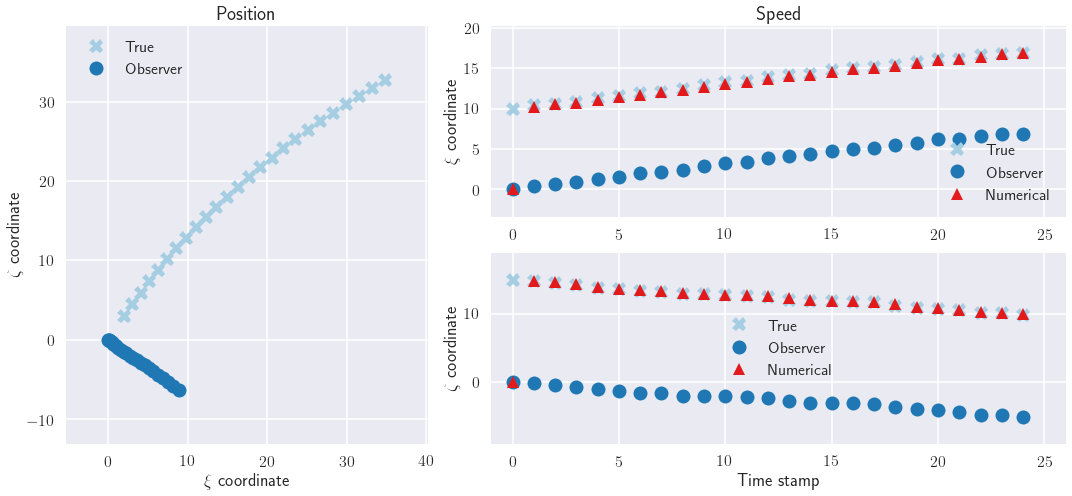
\includegraphics[width=0.8\textwidth]{fig/observer_ex_0}
	 	\caption*{}
	 \end{figure}
 	 
 	 \insertimptext{\bf{Initial errors on speed and position are not corrected over time}}
\end{frame}

\begin{frame}
	\frametitle{A possible solution: Luenberger observer}
	Key idea: use the measured variable for correcting the estimated state
	\vspace{1em}
	
	New equations of the observer
	\vspace{-1em}
	
	\begin{minipage}{0.6\textwidth}
		\begin{align*}
		\hat{\bm{x}}(k+1) &= A_d \hat{\bm{x}}(k) + B_d \bm{u}(k) + 
		\tikz[baseline]{
			\node[fill=blue!10,anchor=base,rounded corners] (corr_term)
			{$L(\bm{y}(k)-\hat{\bm{y}}(k))$};}\\
		\hat{\bm{y}}(k) &= C\hat{\bm{x}}(k) 
		\end{align*}
	\end{minipage}
	\begin{minipage}{0.3\textwidth}
		\tikz[na]\node (descr) {Correcting term}; 
	\end{minipage}
	\begin{tikzpicture}[overlay]
	\path[->](corr_term) edge (descr);
	\end{tikzpicture}\\[2em] 
	\pause
	Consider now the error on the estimated state: $\tilde{\bm{x}}(k)=\bm{x}(k)-\hat{\bm{x}}(k)$. We can write\\[-1.5em]
	\begin{align*}
	\tilde{\bm{x}}(k+1) &=\bm{x}(k+1) - \hat{\bm{x}}(k+1)\\
	 &= A_d \bm{x}(k) + B_d \bm{u}(k) -  
	\left(A_d \hat{\bm{x}}(k) + B_d \bm{u}(k) + L(\bm{y}(k)-\hat{\bm{y}}(k))\right)\\
	 &= A_d \hat{\bm{x}}(k)- LC\bm{x}(k) -  
	A_d \hat{\bm{x}}(k) + LC\hat{\bm{y}}(k)\\
	 &= (A_d - LC)\bm{x}(k)-(A_d-LC) \hat{\bm{x}}(k) \\ 
	 &=(A_d - LC)\tilde{\bm{x}}(k) 
	\end{align*}
	
	%\pause
	%The equation can be rewritten as\hfill \\
	%$\qquad\tilde{\bm{x}}(k)=(A_d-LC)^k\tilde{\bm{x}}(0)$
\end{frame}


\begin{frame}
	\frametitle{A possible solution: Luenberger observer}
	Key idea: use the measured variable for correcting the estimated state
	\vspace{1em}
	
	New equations of the observer
	\vspace{-1em}
	
	\begin{minipage}{0.6\textwidth}
		\begin{align*}
		\hat{\bm{x}}(k+1) &= A_d \hat{\bm{x}}(k) + B_d \bm{u}(k) + 
		\tikz[baseline]{
			\node[fill=blue!10,anchor=base,rounded corners] (corr_term)
			{$L(\bm{y}(k)-\hat{\bm{y}}(k))$};}\\
		\hat{\bm{y}}(k) &= C\hat{\bm{x}}(k) 
		\end{align*}
	\end{minipage}
	\begin{minipage}{0.3\textwidth}
		\tikz[na]\node (descr) {Correcting term}; 
	\end{minipage}
	\begin{tikzpicture}[overlay]
	\path[->](corr_term) edge (descr);
	\end{tikzpicture}\\[2em] 
	\pause
	Consider now the error on the estimated state: $\tilde{\bm{x}}(k)=\bm{x}(k)-\hat{\bm{x}}(k)$. We can write\\[-1.5em]
	\begin{align*}
	\tilde{\bm{x}}(k+1) &=\bm{x}(k+1) - \hat{\bm{x}}(k+1)\\
	&= A_d \bm{x}(k) + B_d \bm{u}(k) -  
	\left(A_d \hat{\bm{x}}(k) + B_d \bm{u}(k) + L(\bm{y}(k)-\hat{\bm{y}}(k))\right)\\
	&= A_d \hat{\bm{x}}(k)- LC\bm{x}(k) -  
	A_d \hat{\bm{x}}(k) + LC\hat{\bm{y}}(k)\\
	&= (A_d - LC)\bm{x}(k)-(A_d-LC) \hat{\bm{x}}(k) \\
	&=\tikz[baseline]{\node[fill=blue!10,anchor=base,rounded corners](dyn_err){$(A_d - LC)$};}\tilde{\bm{x}}(k) \tikz[baseline]{\node[fill=blue!10,anchor=base,rounded corners](no_input){  \phantom{x}};} 
	%&=(A_d - LC)\tilde{\bm{x}}(k) 
	\end{align*}
	
	\tikz[na]\node (comment) {Dynamics of the estimation error};\hspace{1em} \tikz[na]\node (no_input_comment) {Input values have no effect on error dynamics};
	
	\begin{tikzpicture}[overlay]
	\path[->] (no_input_comment) edge (no_input);
	\path[->] (comment) edge (dyn_err);
	\end{tikzpicture}
	
	%\pause
	%The equation can be rewritten as\hfill \\
	%$\qquad\tilde{\bm{x}}(k)=(A_d-LC)^k\tilde{\bm{x}}(0)$
\end{frame}

%\begin{frame}
%	\frametitle{David Luenberger}
%	\begin{columns}
%		\column{0.5\textwidth}
%		\begin{itemize}
%			\item Born September 16, 1937
%			\item \url{https://profiles.stanford.edu/david-luenberger?tab=bio}
%		\end{itemize}
%		\column{0.5\textwidth}
%	\end{columns}
%\end{frame}

\begin{frame}
	\frametitle{Exponential decay - scalar case}
	Focus on the scalar case: $\tilde{x}(k+1)= (a_d-lc)\tilde{x}(k)$	
	%In this case %$x(k)=(a_d-lc)^k
	\begin{itemize}
		%\item The value of the error at time $k=0$ is unknown
		\item If $|a_d-lc|<1$, then $\tilde{x}(k)$ will tend to 0 for all values of $\tilde{x}(0)$
	% 	\item As $k$ grows, it is guaranteed that $|\tilde{x}(k)|$ decreases towards 0
	\end{itemize}

	\begin{figure}[b]
		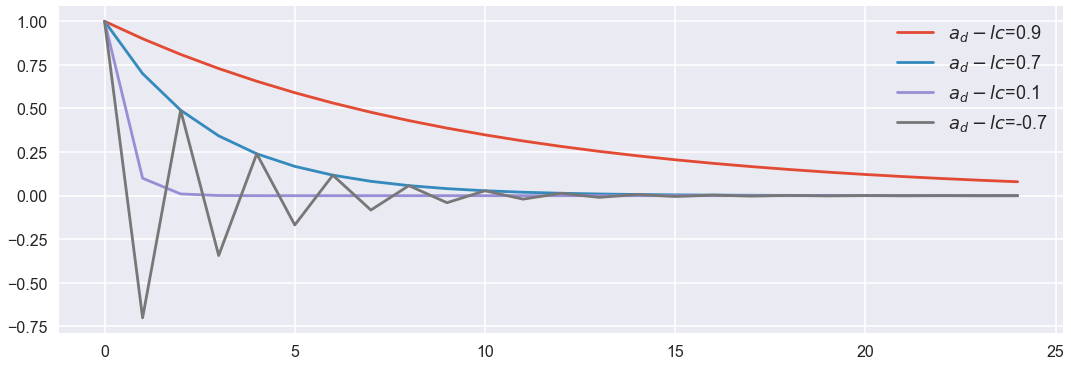
\includegraphics[width=0.9\textwidth]{fig/exponential_decay}
		%\caption*{Exponential decay for different values of $a_d-lc$.}
	\end{figure}
	
	%The non-scalar case requires all eigenvalues of $A_d-LC$ to have absolute value smaller than 1.
	%\takeaway{If $|a_d-lc|<1$, then $\tilde{x}(k)$ tends to 0 for all values $\tilde{x}(0)$}
	
	%\insertimptext{Convergency is guranteed for all values of $\tilde{\bm{x}}(0)$}
	
\end{frame}

\begin{frame}
    \frametitle{Example}
    True and estimated position of the car, along with the true and estimated speed
    %\movie{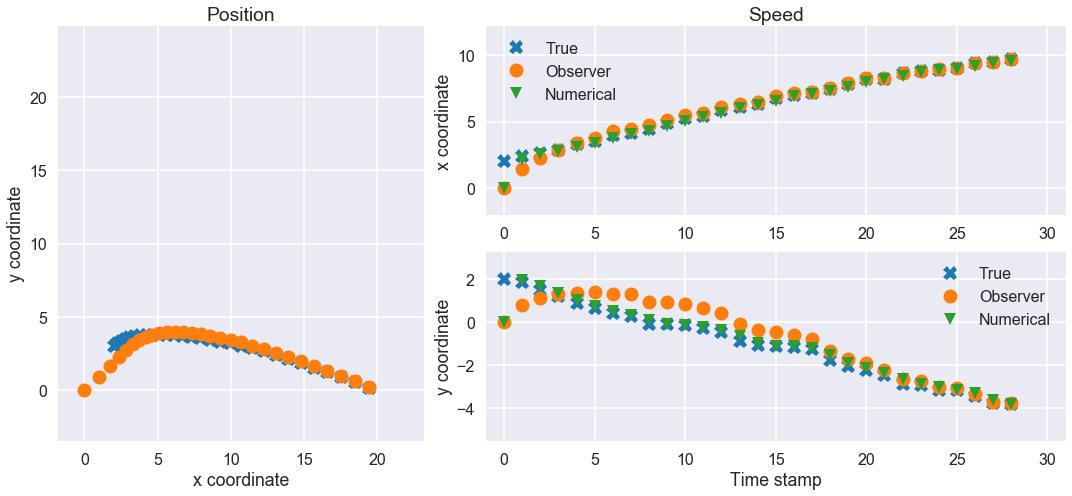
\includegraphics[width=0.8\textwidth]{fig/observer_ex_1}}{video/observer_ex_1.avi}
    \begin{figure}
    	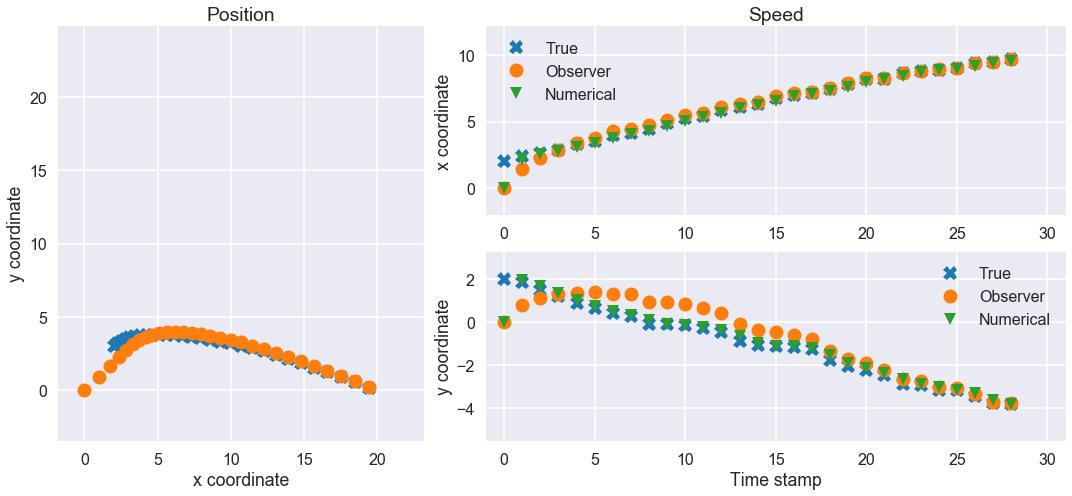
\includegraphics[width=0.9\textwidth]{fig/observer_ex_1}
    \end{figure}
\end{frame}

\begin{frame}
	\frametitle{Estimation with position measurement noise}
	$\xi(k)$ coordinate is affected by noise uniformly distributed between -2 and 2\\
	$\zeta(k)$ coordinate is affected by noise having Gaussian distribution with mean 0 and standard deviation 1
	\begin{figure}
		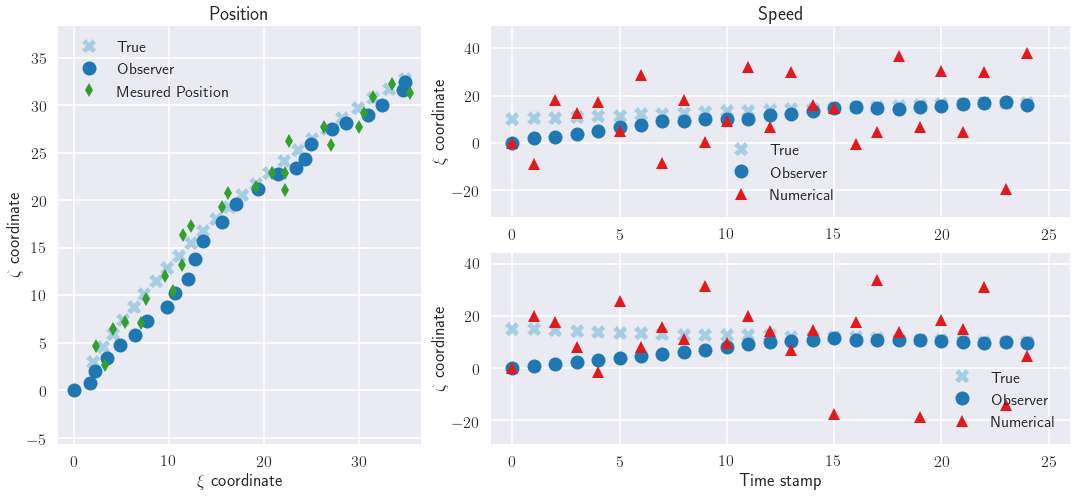
\includegraphics[width=0.9\textwidth]{fig/observer_ex_2}
	\end{figure}
\end{frame}

\begin{frame}
	\frametitle{Estimation with position and acceleration measurement noise}
	$u_1(k)$ measurements are affected by noise with uniform distribution between -2 and 2\\
	$u_2(k)$ measurements are affected by noise with Gaussian distribution with mean 0 and standard deviation 1
	\begin{figure}
		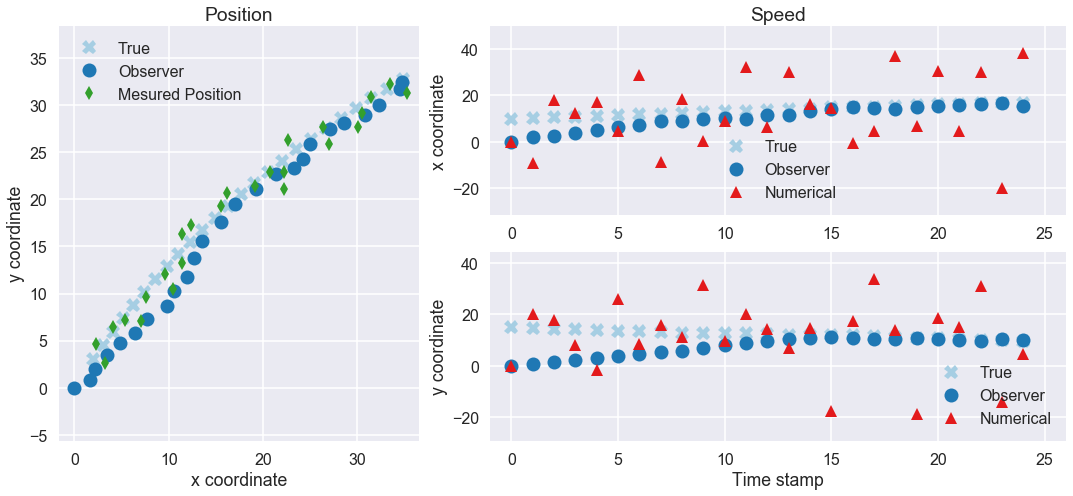
\includegraphics[width=0.9\textwidth]{fig/observer_ex_3}
	\end{figure}
\end{frame}

\begin{frame}
	\frametitle{Summary}
	\begin{itemize}
		\setlength\itemsep{1.5em}
		\item Numerical difference is a viable approach only when measurement noise is negligible
		\item Definition of the observer requires knowledge of the system parameters
		\item Using feedback from the output can compensate initial estimation errors
		\item Multiple gains of the observer can be used
		\item All eigenvalues of $A_d-LC$ have absolute value smaller than 1
		\item For information see, among others, \href{http://cse.lab.imtlucca.it/~bemporad/teaching/ac/pdf/06b-estimator.pdf}{A. Bemporad. State estimation and linear observer}
	\end{itemize}

\insertimptext{\bf{What would it be the best gain?}}
\end{frame}